\documentclass{report}

\input{~/latex/template/preamble.tex}
\input{~/latex/template/macros.tex}

\title{\Huge{Chapter 1 - Differentiation}}
\author{\huge{Matt Warner}}
\date{\huge{}}
\pagestyle{fancy}
\fancyhf{}
\rhead{}
\lhead{\leftmark}
\cfoot{\thepage}
% \usepackage[default]{sourcecodepro}
% \usepackage[T1]{fontenc}


\pgfpagesdeclarelayout{boxed}
{
  \edef\pgfpageoptionborder{0pt}
}
{
  \pgfpagesphysicalpageoptions
  {%
    logical pages=1,%
  }
  \pgfpageslogicalpageoptions{1}
  { 
    border code=\pgfsetlinewidth{1.5pt}\pgfstroke,%
    border shrink=\pgfpageoptionborder,%
    resized width=.95\pgfphysicalwidth,%
    resized height=.95\pgfphysicalheight,%
    center=\pgfpoint{.5\pgfphysicalwidth}{.5\pgfphysicalheight}%
  }%
}

\pgfpagesuselayout{boxed}

\begin{document}
  \maketitle
  \tableofcontents
  \pagebreak
\section{Limits: A numerical and Graphical Approach}
\bigbreak \noindent \bigbreak \noindent
\begin{minipage}{0.44\textwidth}
Consider the pattern formed by the following sequence of numbers	
$$ 0.9, 0.99, 0.999, 0.9999, \text{ and so on}$$
\bigbreak \noindent \bigbreak \noindent
The numbers appear to be getting closer to the number 1, yet never equal 1 exactly. Assuming that the sequence continues in the same manner, we could say that the \textit{limit} of this sequence of numbers is 1. Note that this sequence of numbers approaches 1 ``from the left,'' meaning that all numbers in the sequence are less than the limit, 1. We write $x \rightarrow a $, read ``x approaches a from the left'', to represent a sequence of numbers that approaches $a$ from the left.
\vspace{2mm}

Thus, the sequence 0.9, 0.99,0.999, and so on, is written $x \rightarrow 1$
\end{minipage}
\begin{minipage}{0.55\textwidth}
  \vspace{15mm}

    \incfig[1]{figfig}
    \bigbreak \noindent
\end{minipage}
\bigbreak \noindent \bigbreak \noindent
    The following sequence approaches 1 ``from the right'':
    $$1.1, 1.01,1.001,1.0001,1.00001, \text{ and so on}$$
    \bigbreak \noindent
    We write $ x \rightarrow a^+$, read ``x approaches $a$ from the right'' to represent a sequence of numbers that approaches $a$ from the right.
    \bigbreak \noindent
    Thus, the sequence 1.1, 1.01,1.001,1.0001,1.00001, and so on, is written $x \rightarrow 1^+$
    \bigbreak \noindent
    \bigbreak \bigbreak \noindent
    \ex{}{
      For each sequence, determine its limit, and rewrite the sequence in the form $x \rightarrow a^-$ or $ x \rightarrow a+$
      \bigbreak \noindent
      \begin{enumerate}
        \item $2.24, 2.249, 2.2499, 2.24999,\ldots$ 
        \item $5.51,5.501,5.5001,5.50001,\ldots$
        \item $\frac{1}{2}, \frac{3}{4}, \frac{7}{8}, \frac{15}{16},\frac{31}{32},\frac{63}{64}$
      \end{enumerate}
    }
    \sol{}
  \bigbreak \noindent
  a) $ x \rightarrow 2.25^-$
  \bigbreak \noindent
  b) $x \rightarrow 5.5^+$
  \bigbreak \noindent
  $ c) x \rightarrow 1^-$
\pagebreak
\subsection{Numerical Limits of Functions}
\bigbreak \noindent
\begin{minipage}[t]{0.46\textwidth}
Suppose $f(x) = 2x + 1$, and let $x$ assume the values in the sequence $0.9,0.99,0.999,0.9999,0.99999$, and so on. Evaluating $f(x)$ for each of these values, we have
$$f(0.9) = 2(0.9) + 1 = 2.8$$
$$f(0.99) = 2(0.99) + 1 = 2.98$$
$$f(0.999) = 2(0.999) + 1 = 2.998$$
$$f(0.9999) = 2(0.9999) + 1 = 2.9998 \text{ and so on.}$$
\bigbreak \noindent
As x approaches the number 1 from the left, the sequence of outputs, $f(x)$, approaches the number 3. This is an example of a \textit{left hand limit} and is written
$$\lim_{x\to 1^-}f(x) = 3$$
\end{minipage}
\hspace{.2in}
\begin{minipage}[t]{0.5\textwidth}
  \vspace{-8mm}

  \thm{}{
As $x$ approaches $a$, the limit of $f(x)$ is $L$, where $L$ is a real number, if the left-hand limit exists and the right-hand limit exists and if both limits are $L$. That is,
$$
\text { if } \lim _{x \rightarrow a^{+}} f(x)=\lim _{x \rightarrow a^{-}} f(x)=L \text {, then } \lim _{x \rightarrow a} f(x)=L .
$$
The converse of this theorem is also true: If $\lim _{x \rightarrow a} f(x)=L$, then it follows that $\lim _{x \rightarrow a^{-}} f(x)=L$ and $\lim _{x \rightarrow a^{+}} f(x)=L$
\vspace{4mm}

If the left-hand or right-hand limit does not exist, or if the right-hand and left-hand limits exist but are different, then the limit itself does not exist.
  }
\end{minipage}
\bigbreak \noindent
\nt{
  writing $x\to 1$ with no superscript, $^+$ or $^-$ on 1 indicates that ``x approaches 1 from \textbf{both sides}'' if both the left-hand limit and the right-hand limit exist and are equal to the same real number $L$, then the \textit{general limit} (or simply, the \textit{limit}) is $L$. In the above example, since the limit as x approaches from both sides is the same. You can ingore writing the superscripts. This leads to theorem 1.
}
\bigbreak \noindent\bigbreak \noindent
\subsection{Graphical Limits}
\bigbreak \noindent
To view limits Graphically, we let $f(x) = 2x+3$ and select x-values that get close to 4. In the table and graph below, we see that as input values approach 4 from the left (that is, are less than 4), output values approach 11, and as input values approach 4 from the right (that is, are greater than 4), output values also approach 11. Thus, we say;
\bigbreak \noindent
As x approaches 4 from either side, the function $f(x) = 2x+3$ approaches 11.
\begin{figure}[ht]
    \centering
    \incfig[1]{lim}
\end{figure}
\bigbreak \noindent
\begin{center}
\begin{tabular}{|c|r|r|r|r|r|r|r|}
  \hline
$x$ & 3.9 & 3.99 & 3.999 & 4 & 4.001 & 4.01 & 4.1 \\
\hline$f(x)$ & 10.8 & 10.98 & 10.998 & 11 & 11.002 & 11.02 & 11.2 \\
\hline
\end{tabular}
\end{center}

\pagebreak
\ex{}{
  Let $f(x) = -3x + 4$. Find the following limits
  \begin{enumerate}
    \item $\displaystyle\lim_{x\to 2^-}f(x)$
    \item $\displaystyle\lim_{x\to2^+}f(x)$
    \item $\displaystyle\lim_{x\to2}f(x)$

      \vspace{3mm}


  \end{enumerate}
}
\bigbreak \noindent
\sol{}
\bigbreak \noindent

$$\displaystyle\lim_{x\to2^-}-3x+4$$
\noindent set x = 2
$$\displaystyle\lim_{x\to2^-}-3(2) +4 = -2$$
\vspace{2mm}

\noindent
Thus the limit of $f(x)$ as x approaches 2 is $-2$
\bigbreak \noindent
The same proccess can be applied to the limit of f(x) as x approaches to the right, since we get the same answer for both, we conclude that
$$\displaystyle\lim_{x\to 2}f(x) = -2$$
\nt{
  The method used above is a shortcut and is only permissible under certain conditions, This will be discussed in the next section. The numerical apporach to finding the limit can be found below.
}
\bigbreak \noindet
a) We choose values of $x$ that approach 2 from the left, and evaluate $f(x)$ :
$$
\begin{aligned}
f(1.9) & =-3(1.9)+4=-1.7, \\
f(1.99) & =-3(1.99)+4=-1.97, \\
f(1.999) & =-3(1.999)+4=-1.997, \text { and so on. }
\end{aligned}
$$
We see that as $x$ approaches 2 from the left, the function values approach -2 . Thus, we have a left-hand limit, $\lim _{x \rightarrow 2} f(x)=-2$
\bigbreak 
b) We choose values of $x$ that approach 2 from the right, and evaluate $f(x)$ :
$$
\begin{aligned}
f(2.1) & =-3(2.1)+4=-2.3, \\
f(2.01) & =-3(2.01)+4=-2.03, \\
f(2.001) & =-3(2.001)+4=-2.003, \text { and so on. }
\end{aligned}
$$
We see that as $x$ approaches 2 from the right, the function values approach -2 . Thus, we have a right-hand limit, $\lim _{x \rightarrow 2^{+}} f(x)=-2$.
\bigbreak \noindent
c) Since the left-hand limit and the right-hand limit exist and are both equal to -2 , we conclude that the limit as $x$ approaches 2 exists and is -2 : $\lim _{x \rightarrow 2} f(x)=-2$.
\pagebreak
\ex{}{
  Let $f(x) = \frac{x^2-1}{x-1}$. Find $\displaystyle\lim_{x\to 1}f(x)$
}
\sol
\bigbreak \noindent
For this question, note that we cannot directly find the limit by setting $x = 1$ (direct substitution), since that would give us a zero in the denominator, which is no good.
\bigbreak
\noindent Thus, we use a numerical approach for this question.
\bigbreak \noindent \bigbreak \noindent
\hspace{25mm}\begin{minipage}{0.45\textwidth}
  \hspace{2em}
  left-hand limit
  \vspace{2mm}

\begin{tabular}{|c|l|}
\hline$x \rightarrow 1^{-}(x<1)$ & $f(x)$ \\
\hline 0.9 & 1.9 \\
0.99 & 1.99 \\
0.999 & 1.999 \\
\hline
\end{tabular}
\vspace{4mm}

\hspace{8mm}$\displaystyle\lim_{x\to 1^-}f(x) = 2$
\end{minipage}
\begin{minipage}{0.39\textwidth}
  \hspace{6mm}right-hand limit
  \vspace{2mm}

	\begin{tabular}{|c|l|}
\hline$x \rightarrow 1^{+}(x>1)$ & $f(x)$ \\
\hline 1.1 & 2.1 \\
1.01 & 2.01 \\
1.001 & 2.001 \\
\hline
\end{tabular}
\vspace{4mm}

\hspace{10mm}$\displaystyle\lim_{x\to 1^+ }f(x) = 2$
\end{minipage}
\bigbreak \noindent
Since the left-hand limit and right-hand limit exist and are equal, we conclude that the limit of $f(x)$ as $x$ approaches 1 is
$$\displaystyle\lim_{x\to 1}f(x) = 2$$
\bigbreak \noindent
Thus, the graph of $f(x) = \frac{x^2-1}{x-1}$ is the line given by $f(x) = x + 1$ where the point corresponding to x = 1 has been removed.
\bigbreak \noindent
The graph has a ``hole'' at the point (1,2). Thus, even though the function is not defined at x = 1, the limit \textit{does} exist as $x\to 1$, and its value is 2.
\begin{figure}[ht]
    \centering
    \incfig[1]{limlim}
    %\caption{limlim}
    %\label{fig:limlim}
\end{figure}
\bigbreak \noindent
To Summarize:
\begin{enumerate}
  \item When x = 1 exactly, $f(x)$ is undefined. The value $x = 1$ is not in the domain of $f$.
  \item When x approaches 1 from both sides, the output values approach 2.
\end{enumerate}
\pagebreak
\ex{}{
  Consider the function $H$ given by
 $$H(x)= \begin{cases}2 x+2, & \text { for } x<1 \\ 2 x-4, & \text { for } x \geq 1\end{cases}$$
 \bigbreak \noindent
 Find $\displaystyle\lim_{x\to 1}H(x)$
}
\sol{}
\bigbreak \noindent
\begin{figure}[ht]
\centering
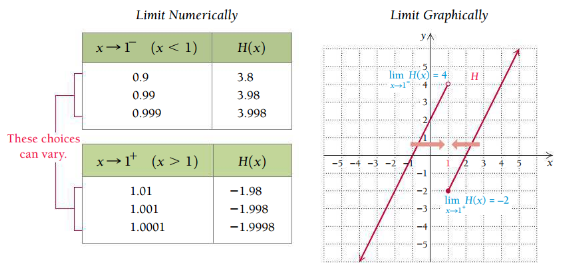
\includegraphics[width=0.7\textwidth]{ /home/mattw/niu/Math211/figures/ksnip_20230921-181045.png }
\end{figure}
\bigbreak \noindent
As input x approach 1 from the left (see the upper table), outputs $H(x)$ approach 4.
Thus, the left-hand limit is 4. That is,
$$\displaystyle\lim_{x\to 1+}H(x) = -2$$
\bigbreak \noindent
As input x approach 1 from the right (see the upper table), outputs H(x) approach -2. Thus the right-hand limit is -2. That is,
$$\displaystyle\lim_{x\to 1+}H(x) = -2$$
\bigbreak \noindent
Since the left-hand limit, 4, is not the same as the right hand limit, -2, we say that
$$\displaystyle\lim_{x\to 1}H(x) \text{ Does not exist (DNE)}$$
\bigbreak \noindent \bigbreak \noindent
\subsection{The wall Method}
\bigbreak \noindent
An alternative approach for Example 1.4 is to draw a ``wall'' at x = 1, as shown in blue on the graph to the left below. We then trace the graph from left to right with a pencil until we hit the wall and mark the location with an x, assuming it can be determined. Then we trace the graph from right to left until we hit the wall and mark that location with an x. If the locations are not the same, as shown in the graph on the left, a limit does not exist. Thus, for Example 4,
$$\displaystyle\lim_{x\to 1}H(x) \text{ does not exist} $$
\pagebreak
\begin{figure}[ht]
\centering
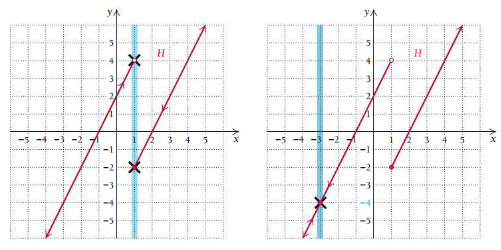
\includegraphics[width=0.6\textwidth]{ /home/mattw/niu/Math211/figures/ksnip_20230921-191506.png }
\caption*{wall method}
\end{figure}
\bigbreak \noindent
However, for any other value a, $\displaystyle\lim_{x\to a }H(x)$ does exist. For example, as x approaches -3, we see in the graph to the right that the wall method gives -4 whether -3 is approached from the left or from the right. Thus,
$$\displaystyle\lim_{x\to -3 }H(x) = -4$$
\bigbreak \noindent
\ex{}{
  Consider the piecewise function defined as follows:
 $$
G(x)= \begin{cases}5, & \text { for } x=1 \\ x+1, & \text { for } x \neq 1\end{cases}
$$ 
\bigbreak \noindent
Graph the function, and find each of the following:
\bigbreak \noindent
$$\text{a) } G(1)\hspace{10mm} \text{b) } \displaystyle\lim_{x\to 1}G(x)$$
}
\sol{}
\bigbreak \noindent
The graph of G follows.
\begin{figure}[ht]
    \centering
    \incfig[1]{fg}
    %\caption{fg}
    %\label{fig:fg}
\end{figure}
\bigbreak \noindent
From the definition of G, we see that
$$G(1) = 5$$
\pagebreak

\noindent b) As inputs x approach 1 from the left, outputs $G(x)$ approach 2, so the limit from the left is 2. As inputs x approach 1 from the right, outputs G(x) also approach 2, so the limit from the right is 2. Both limits are the same, so
$$\displaystyle\lim_{x\to 1}G(x) = 2$$
\bigbreak \noindent
\nt{
  Note that the limit, 2, is not the same as the function value of 1.
}
\begin{figure}[ht]
\centering
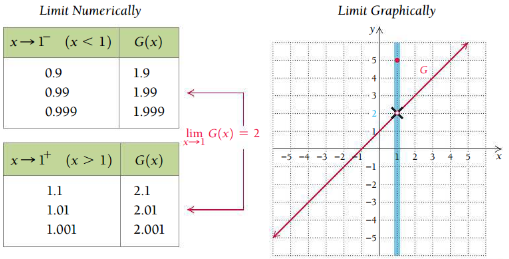
\includegraphics[width=0.65\textwidth]{ /home/mattw/niu/Math211/figures/IV.png }
\end{figure}
\bigbreak \noindent \bigbreak \noindent
\subsection{Limits Involving Infinity}
\bigbreak \noindent
Limits also help us understand the role of infinity with respect to some functions.
\bigbreak \noindent
\ex{}{
  \Let $f(x) = \frac{1}{x-2}$
  \bigbreak \noindent
  \begin{enumerate}
    \item Find $\displaystyle\lim_{x\to 2^-}f(x)$
    \item Find $\displaystyle\lim_{x\to 2^+}f(x)$
    \item Does $\displaystyle\lim_{x\to 2}f(x)$ exist? Why or why not?
  \end{enumerate}
}
\sol
\bigbreak \noindent
a) \centerline{$}
\end{document}

